%% generated by python/export_effect_ledger.py
%% sweeps: 2026-10-02-paper, GNvpro top-up on the T=1 degree axis; commit 259ce29
%% blue interval: median seed geometric SD of that row and optimizer;
% pale markers fall inside it. Overall median 1.142 over 152 combinations.
%% "own" counts each marker against its own seed spread instead.
%%   monomial on $[0,T]$ / monomial on $[-1,1]$ [$T{=}10$] Adam     n= 6 median 5.187 gsd 1.154 beyond 6/6 (own 5/6)
%%   monomial on $[0,T]$ / monomial on $[-1,1]$ [$T{=}10$] GNvpro   n= 6 median 3.073 gsd 1.444 beyond 6/6 (own 6/6)
%%   monomial on $[0,T]$ / monomial on $[-1,1]$ [$T{=}5$] Adam      n= 6 median 1.375 gsd 1.133 beyond 6/6 (own 6/6)
%%   monomial on $[0,T]$ / monomial on $[-1,1]$ [$T{=}5$] GNvpro    n= 6 median 2.673 gsd 1.350 beyond 6/6 (own 6/6)
%%   monomial on $[0,T]$ / monomial on $[-1,1]$ [$T{=}1$] Adam      n= 6 median 1.031 gsd 1.140 beyond 1/6 (own 1/6)
%%   monomial on $[0,T]$ / monomial on $[-1,1]$ [$T{=}1$] GNvpro    n= 6 median 0.986 gsd 1.187 beyond 2/6 (own 0/6)
%%   Legendre, $D{=}11$ / Legendre, $D{=}0$ [all] Adam              n= 6 median 0.768 gsd 1.115 beyond 5/6 (own 5/6)
%%   Legendre, $D{=}11$ / Legendre, $D{=}0$ [all] GNvpro            n= 6 median 1.027 gsd 1.182 beyond 1/6 (own 0/6)
%%   Legendre, $D{=}0$ / unconstrained [ELM] Adam                   n= 2 median 1.019 gsd 1.039 beyond 0/2 (own 0/2)
%%   Legendre, $D{=}0$ / unconstrained [ELM] GNvpro                 n= 2 median 1.001 gsd 1.060 beyond 0/2 (own 0/2)
%%   " / " [CDR] Adam                                               n= 2 median 1.526 gsd 1.144 beyond 2/2 (own 2/2)
%%   " / " [CDR] GNvpro                                             n= 2 median 1.012 gsd 1.438 beyond 0/2 (own 0/2)
%%   " / " [DCR] Adam                                               n= 2 median 0.743 gsd 1.115 beyond 2/2 (own 2/2)
%%   " / " [DCR] GNvpro                                             n= 2 median 0.729 gsd 1.230 beyond 2/2 (own 2/2)
%%   Legendre, $D{=}4$--$8$ / monomial, $D{=}4$--$8$ [CDR] Adam     n=10 median 0.882 gsd 1.123 beyond 6/10 (own 4/10)
%%   Legendre, $D{=}4$--$8$ / monomial, $D{=}4$--$8$ [CDR] GNvpro   n=10 median 0.980 gsd 1.128 beyond 2/10 (own 1/10)
%%   Legendre, $D{=}3$ / monomial, $D{=}3$ [all] Adam               n=18 median 1.007 gsd 1.144 beyond 2/18 (own 2/18)
%%   Legendre, $D{=}3$ / monomial, $D{=}3$ [all] GNvpro             n=18 median 0.994 gsd 1.270 beyond 1/18 (own 0/18)
%%   single precision / double precision [CDR] Adam                 n=18 median 1.000 gsd 1.100 beyond 0/18 (own 0/18)
%%   single precision / double precision [CDR] GNvpro               n=18 median 0.998 gsd 1.297 beyond 0/18 (own 0/18)
\documentclass[tikz]{standalone}
\usepackage{pgfplots}
\pgfplotsset{compat=1.18}
\definecolor{mycolor5}{rgb}{1.0,0.03,0.0}
\definecolor{bandblue}{rgb}{0.10,0.32,0.72}
\begin{document}
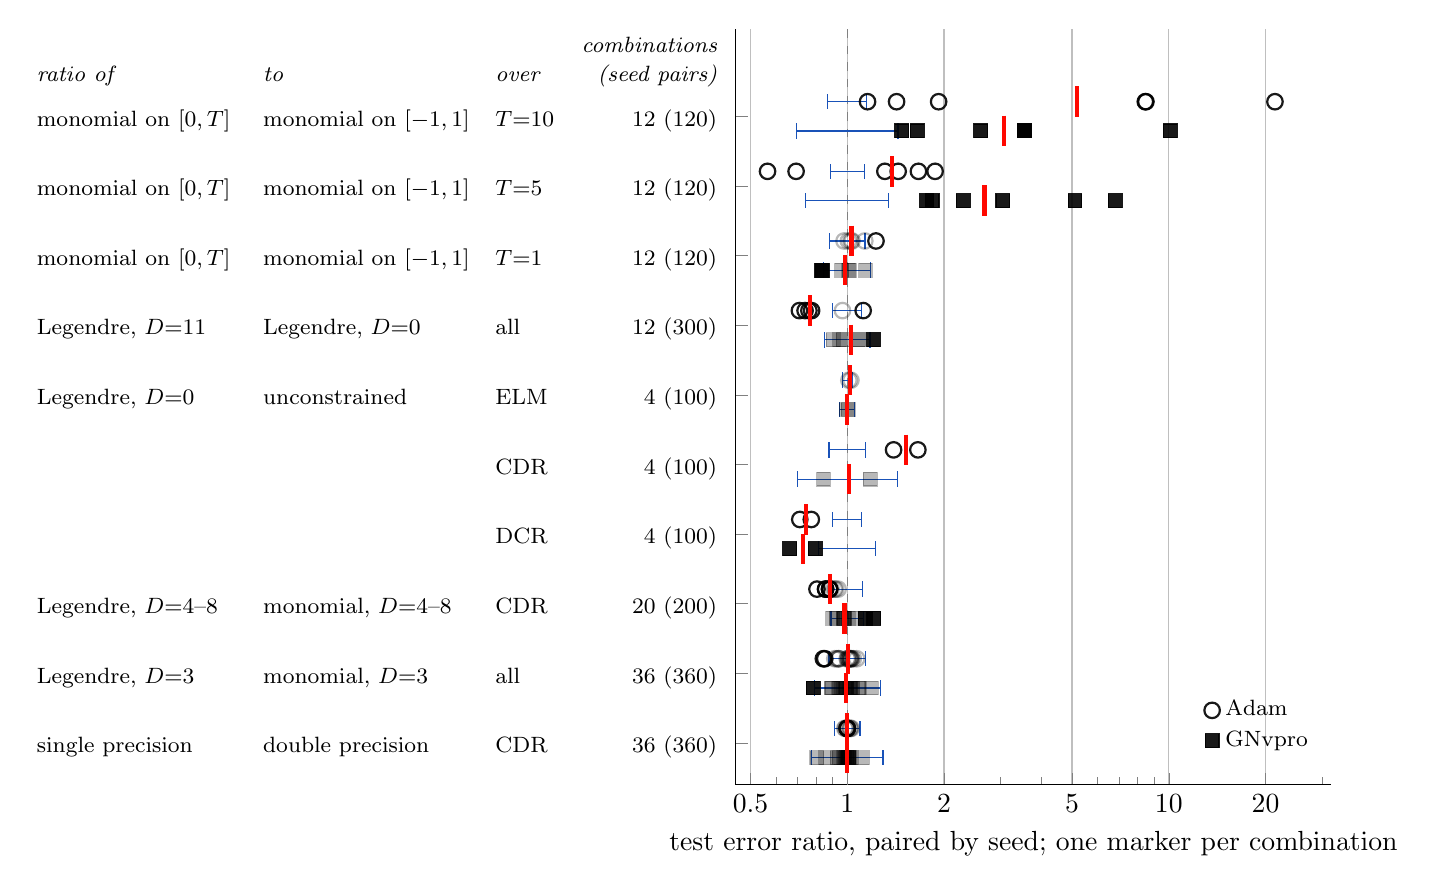
\begin{tikzpicture}
\begin{axis}[width=3.6in,height=4.4in,xmode=log,
  xlabel={test error ratio, paired by seed; one marker per combination},
  xmin=0.45,xmax=32,ymin=0.4,ymax=11.25,
  xtick={0.5,1,2,5,10,20},
  xticklabels={$0.5$,$1$,$2$,$5$,$10$,$20$},
  minor xtick={0.6,0.7,0.8,0.9,3,4,6,7,8,9,30},
  ytick={10,9,8,7,6,5,4,3,2,1},yticklabels={},
  legend style={at={(0.985,0.03)},anchor=south east,draw=none,fill=none,
    font=\footnotesize,legend cell align=left},
  xmajorgrids,axis y line*=left,axis x line*=bottom,
  clip=false]
\addplot[dashed,gray,mark=none,forget plot] coordinates {(1,0.4) (1,11.25)};
\draw[bandblue,|-|,line width=0.4pt] (axis cs:0.8668,10.21) -- (axis cs:1.1537,10.21);
\draw[bandblue,|-|,line width=0.4pt] (axis cs:0.6923,9.79) -- (axis cs:1.4444,9.79);
\draw[bandblue,|-|,line width=0.4pt] (axis cs:0.8829,9.21) -- (axis cs:1.1327,9.21);
\draw[bandblue,|-|,line width=0.4pt] (axis cs:0.7406,8.79) -- (axis cs:1.3502,8.79);
\draw[bandblue,|-|,line width=0.4pt] (axis cs:0.8768,8.21) -- (axis cs:1.1405,8.21);
\draw[bandblue,|-|,line width=0.4pt] (axis cs:0.8423,7.79) -- (axis cs:1.1872,7.79);
\draw[bandblue,|-|,line width=0.4pt] (axis cs:0.8965,7.21) -- (axis cs:1.1154,7.21);
\draw[bandblue,|-|,line width=0.4pt] (axis cs:0.8460,6.79) -- (axis cs:1.1820,6.79);
\draw[bandblue,|-|,line width=0.4pt] (axis cs:0.9628,6.21) -- (axis cs:1.0386,6.21);
\draw[bandblue,|-|,line width=0.4pt] (axis cs:0.9435,5.79) -- (axis cs:1.0599,5.79);
\draw[bandblue,|-|,line width=0.4pt] (axis cs:0.8739,5.21) -- (axis cs:1.1443,5.21);
\draw[bandblue,|-|,line width=0.4pt] (axis cs:0.6956,4.79) -- (axis cs:1.4377,4.79);
\draw[bandblue,|-|,line width=0.4pt] (axis cs:0.8972,4.21) -- (axis cs:1.1146,4.21);
\draw[bandblue,|-|,line width=0.4pt] (axis cs:0.8132,3.79) -- (axis cs:1.2298,3.79);
\draw[bandblue,|-|,line width=0.4pt] (axis cs:0.8902,3.21) -- (axis cs:1.1233,3.21);
\draw[bandblue,|-|,line width=0.4pt] (axis cs:0.8868,2.79) -- (axis cs:1.1276,2.79);
\draw[bandblue,|-|,line width=0.4pt] (axis cs:0.8743,2.21) -- (axis cs:1.1438,2.21);
\draw[bandblue,|-|,line width=0.4pt] (axis cs:0.7872,1.79) -- (axis cs:1.2703,1.79);
\draw[bandblue,|-|,line width=0.4pt] (axis cs:0.9088,1.21) -- (axis cs:1.1003,1.21);
\draw[bandblue,|-|,line width=0.4pt] (axis cs:0.7711,0.79) -- (axis cs:1.2969,0.79);
\addlegendimage{only marks,mark=o,mark size=2.8pt,mark options={line width=0.8pt},color=black,opacity=0.9}
\addlegendentry{Adam}
\addlegendimage{only marks,mark=square*,mark size=2.5pt,color=black,opacity=0.9}
\addlegendentry{GNvpro}
\addplot[only marks,mark=o,mark size=2.8pt,mark options={line width=0.8pt},color=black,opacity=0.28,forget plot] coordinates {(0.9773,8.21) (1.0079,8.21) (1.0264,8.21) (1.0352,8.21) (1.1340,8.21) (0.9664,7.21) (1.0116,6.21) (1.0267,6.21) (0.8910,3.21) (0.9115,3.21) (0.9191,3.21) (0.9368,3.21) (0.9146,2.21) (0.9271,2.21) (0.9384,2.21) (0.9409,2.21) (0.9429,2.21) (0.9996,2.21) (1.0024,2.21) (1.0110,2.21) (1.0112,2.21) (1.0201,2.21) (1.0205,2.21) (1.0254,2.21) (1.0275,2.21) (1.0318,2.21) (1.0448,2.21) (1.0704,2.21) (0.9827,1.21) (0.9880,1.21) (0.9977,1.21) (0.9994,1.21) (0.9999,1.21) (0.9999,1.21) (1.0000,1.21) (1.0000,1.21) (1.0000,1.21) (1.0000,1.21) (1.0000,1.21) (1.0001,1.21) (1.0004,1.21) (1.0009,1.21) (1.0015,1.21) (1.0153,1.21) (1.0223,1.21) (1.0291,1.21)};
\addplot[only marks,mark=o,mark size=2.8pt,mark options={line width=0.8pt},color=black,opacity=0.9,forget plot] coordinates {(1.1564,10.21) (1.4237,10.21) (1.9241,10.21) (8.4507,10.21) (8.4899,10.21) (21.3873,10.21) (0.5651,9.21) (0.6934,9.21) (1.3094,9.21) (1.4400,9.21) (1.6650,9.21) (1.8761,9.21) (1.2285,8.21) (0.7101,7.21) (0.7394,7.21) (0.7602,7.21) (0.7749,7.21) (1.1209,7.21) (1.3936,5.21) (1.6586,5.21) (0.7121,4.21) (0.7732,4.21) (0.8052,3.21) (0.8560,3.21) (0.8571,3.21) (0.8808,3.21) (0.8808,3.21) (0.8828,3.21) (0.8427,2.21) (0.8514,2.21)};
\addplot[only marks,mark=square*,mark size=2.5pt,color=black,opacity=0.28,forget plot] coordinates {(0.9622,7.79) (1.0094,7.79) (1.0140,7.79) (1.1393,7.79) (0.9054,6.79) (0.9456,6.79) (0.9704,6.79) (1.0841,6.79) (1.0843,6.79) (0.9935,5.79) (1.0080,5.79) (0.8440,4.79) (1.1803,4.79) (0.9000,2.79) (0.9228,2.79) (0.9725,2.79) (0.9763,2.79) (0.9789,2.79) (0.9818,2.79) (1.0094,2.79) (1.0596,2.79) (0.8915,1.79) (0.8988,1.79) (0.9402,1.79) (0.9458,1.79) (0.9614,1.79) (0.9735,1.79) (0.9846,1.79) (0.9929,1.79) (0.9943,1.79) (0.9962,1.79) (1.0191,1.79) (1.0271,1.79) (1.0293,1.79) (1.0390,1.79) (1.0818,1.79) (1.0884,1.79) (1.1891,1.79) (0.8048,0.79) (0.8576,0.79) (0.9293,0.79) (0.9459,0.79) (0.9553,0.79) (0.9743,0.79) (0.9835,0.79) (0.9944,0.79) (0.9973,0.79) (0.9994,0.79) (1.0056,0.79) (1.0072,0.79) (1.0078,0.79) (1.0111,0.79) (1.0125,0.79) (1.0132,0.79) (1.0304,0.79) (1.1150,0.79)};
\addplot[only marks,mark=square*,mark size=2.5pt,color=black,opacity=0.9,forget plot] coordinates {(1.4759,9.79) (1.6510,9.79) (2.5983,9.79) (3.5477,9.79) (3.5553,9.79) (10.1011,9.79) (1.7682,8.79) (1.8357,8.79) (2.2970,8.79) (3.0480,8.79) (5.1084,8.79) (6.8201,8.79) (0.8321,7.79) (0.8361,7.79) (1.2074,6.79) (0.6623,3.79) (0.7952,3.79) (1.1380,2.79) (1.2107,2.79) (0.7838,1.79)};
\addplot[only marks,mark=|,mark size=5.5pt,line width=1.5pt,color=mycolor5,forget plot] coordinates {(5.1874,10.21) (3.0730,9.79) (1.3747,9.21) (2.6725,8.79) (1.0308,8.21) (0.9858,7.79) (0.7676,7.21) (1.0273,6.79) (1.0191,6.21) (1.0008,5.79) (1.5261,5.21) (1.0121,4.79) (0.7427,4.21) (0.7287,3.79) (0.8818,3.21) (0.9804,2.79) (1.0067,2.21) (0.9936,1.79) (1.0000,1.21) (0.9984,0.79)};
\node[anchor=base west,font=\footnotesize\itshape] at (axis description cs:-1.190,0.9309) {ratio of};
\node[anchor=base west,font=\footnotesize\itshape] at (axis description cs:-0.810,0.9309) {to};
\node[anchor=base west,font=\footnotesize\itshape] at (axis description cs:-0.420,0.9309) {over};
\node[anchor=base east,font=\footnotesize\itshape] at (axis description cs:-0.015,0.9696) {combinations};
\node[anchor=base east,font=\footnotesize\itshape] at (axis description cs:-0.015,0.9309) {(seed pairs)};
\node[anchor=base west,font=\footnotesize] at (axis description cs:-1.190,0.8719) {monomial on $[0,T]$};
\node[anchor=base west,font=\footnotesize] at (axis description cs:-0.810,0.8719) {monomial on $[-1,1]$};
\node[anchor=base west,font=\footnotesize] at (axis description cs:-0.420,0.8719) {$T{=}10$};
\node[anchor=base east,font=\footnotesize] at (axis description cs:-0.015,0.8719) {12 (120)};
\node[anchor=base west,font=\footnotesize] at (axis description cs:-1.190,0.7797) {monomial on $[0,T]$};
\node[anchor=base west,font=\footnotesize] at (axis description cs:-0.810,0.7797) {monomial on $[-1,1]$};
\node[anchor=base west,font=\footnotesize] at (axis description cs:-0.420,0.7797) {$T{=}5$};
\node[anchor=base east,font=\footnotesize] at (axis description cs:-0.015,0.7797) {12 (120)};
\node[anchor=base west,font=\footnotesize] at (axis description cs:-1.190,0.6876) {monomial on $[0,T]$};
\node[anchor=base west,font=\footnotesize] at (axis description cs:-0.810,0.6876) {monomial on $[-1,1]$};
\node[anchor=base west,font=\footnotesize] at (axis description cs:-0.420,0.6876) {$T{=}1$};
\node[anchor=base east,font=\footnotesize] at (axis description cs:-0.015,0.6876) {12 (120)};
\node[anchor=base west,font=\footnotesize] at (axis description cs:-1.190,0.5954) {Legendre, $D{=}11$};
\node[anchor=base west,font=\footnotesize] at (axis description cs:-0.810,0.5954) {Legendre, $D{=}0$};
\node[anchor=base west,font=\footnotesize] at (axis description cs:-0.420,0.5954) {all};
\node[anchor=base east,font=\footnotesize] at (axis description cs:-0.015,0.5954) {12 (300)};
\node[anchor=base west,font=\footnotesize] at (axis description cs:-1.190,0.5032) {Legendre, $D{=}0$};
\node[anchor=base west,font=\footnotesize] at (axis description cs:-0.810,0.5032) {unconstrained};
\node[anchor=base west,font=\footnotesize] at (axis description cs:-0.420,0.5032) {ELM};
\node[anchor=base east,font=\footnotesize] at (axis description cs:-0.015,0.5032) {4 (100)};
\node[anchor=base west,font=\footnotesize] at (axis description cs:-0.420,0.4111) {CDR};
\node[anchor=base east,font=\footnotesize] at (axis description cs:-0.015,0.4111) {4 (100)};
\node[anchor=base west,font=\footnotesize] at (axis description cs:-0.420,0.3189) {DCR};
\node[anchor=base east,font=\footnotesize] at (axis description cs:-0.015,0.3189) {4 (100)};
\node[anchor=base west,font=\footnotesize] at (axis description cs:-1.190,0.2267) {Legendre, $D{=}4$--$8$};
\node[anchor=base west,font=\footnotesize] at (axis description cs:-0.810,0.2267) {monomial, $D{=}4$--$8$};
\node[anchor=base west,font=\footnotesize] at (axis description cs:-0.420,0.2267) {CDR};
\node[anchor=base east,font=\footnotesize] at (axis description cs:-0.015,0.2267) {20 (200)};
\node[anchor=base west,font=\footnotesize] at (axis description cs:-1.190,0.1346) {Legendre, $D{=}3$};
\node[anchor=base west,font=\footnotesize] at (axis description cs:-0.810,0.1346) {monomial, $D{=}3$};
\node[anchor=base west,font=\footnotesize] at (axis description cs:-0.420,0.1346) {all};
\node[anchor=base east,font=\footnotesize] at (axis description cs:-0.015,0.1346) {36 (360)};
\node[anchor=base west,font=\footnotesize] at (axis description cs:-1.190,0.0424) {single precision};
\node[anchor=base west,font=\footnotesize] at (axis description cs:-0.810,0.0424) {double precision};
\node[anchor=base west,font=\footnotesize] at (axis description cs:-0.420,0.0424) {CDR};
\node[anchor=base east,font=\footnotesize] at (axis description cs:-0.015,0.0424) {36 (360)};
\end{axis}
\end{tikzpicture}
\end{document}
